%
% Macros para simplificar a demonstração dos erros
%

\newcommand{\errado}[1]{\textbf{\textcolor{red}{#1}}}
\newcommand{\certo}[1]{\textbf{\textcolor{ForestGreen}{#1}}}
% Para não confundir com os exemplos de certo e errado não são colocados os pontos e ponto e virgula dos itens
\newcommand{\erradocerto}[3]{\item #1:\begin{itemize}
    \item \errado{#2}
    \item \certo{#3}
\end{itemize}}
\newcommand{\erradoerradocerto}[4]{\item #1:\begin{itemize}
    \item \errado{#2}
    \item \errado{#3}
    \item \certo{#4}
\end{itemize}}
\newcommand{\erradocertocerto}[4]{\item #1:\begin{itemize}
    \item \errado{#2}
    \item \certo{#3}
    \item \certo{#4}
\end{itemize}}



% Para demonstrar o erro nome deve ser igual entre o capitulo e a seção, então fica em um comando para facilitar
\newcommand{\nomeDoCapitulo}{Erros comuns em documentos}
\chapter{\nomeDoCapitulo}
\label{erros-comuns-capitulo}

% Não colocar nada aqui pois é uma demonstração de erro comum
\explicacaoErro{Passando de capítulo para seção sem texto}
\explicacaoErro{Seção com mesmo nome do capítulo}

\section{\nomeDoCapitulo}
\label{erros-comuns}

% Não colocar nada aqui pois é uma demonstração de erro comum
\explicacaoErro{Passando de seção para subseção sem texto}

\subsection{Subseção sem texto entre o item anterior}
\label{erros-comuns-sub1}


% Tem um erro proposital aqui duplicando "seção" que é escrita também pelo autoref, esse erro é citado em um paragrafo na sequencia....
Essa seção \autoref{erros-comuns} demonstra alguns dos erros mais comuns que percebemos em trabalhos de alunos. Alguns itens errados são apresentados em \errado{vermelho} e corretos em \certo{verde}, mas devido a formatação dos links pode haver uma variação. Lembre que a utilização de cores não é recomendada no documento acadêmico, elas foram utilizadas nesse documento para facilitar a demonstração dos erros.

Além desses erros é comum encontrar a falta de correção ortográfica e utilização errada de palavras. É importante sempre utilizar a correção ortográfica e ainda fazer a revisão por diversas pessoas para evitar erros de português, a língua portuguesa tem palavras parecidas com sentidos diferente, cuidado com a utilização dos acentos e pontuação como pode ser visto claramente em  \autoref{fig_portugues_amador}.

No \autoref{revisao-de-textos} é apresentado um processo simples para revisão de documentos que detecta a maior parte dos erros descritos neste documento.

% erro proposital que esta no inicio da seção
Você percebeu que essa seção iniciou com um erro e que esse erro não está indicado em vermelho ?


\begin{figure}[htb]
    \centering
	\caption{\label{fig_portugues_amador}Português não é para amador}
	\frame{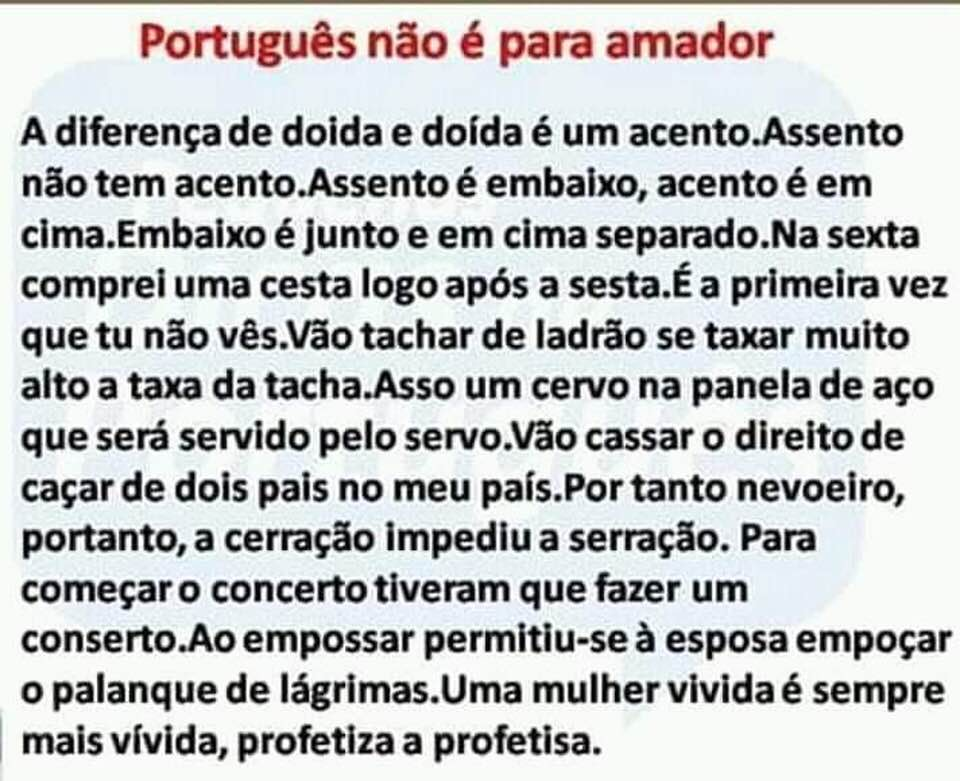
\includegraphics[width=0.9\textwidth]{erros/portugues_nao_eh_para_amador.jpg}}
	\fonte{Autor Desconhecido.}
\end{figure}


Exemplos de erros encontrados em documentos das disciplinas de projetos são apresentados nas seções seguintes. E existem dicas adicionais sobre textos disponíveis em \url{https://dicas.ivanfm.com/aulas/textos/}.


\todo[inline]{Separar esses itens em grupos mais específicos}

\subsection{Subseção com titulo que tenta ser introdução:}
\label{erros-titulo-dois-pontos}
\errado{Colocar um título de seção/seção com dois pontos no final tentando indicar uma introdução para o texto da seção.}
\explicacaoErro{Além disso essa seção tem somente um pequeno parágrafo, ver \autoref{erros-formatacao-docto}}

\subsection{Erros comuns de texto}
    
\begin{itemize}
    \erradocerto{Abreviação ou nomes incompletos dos participantes do trabalho e/ou professores na capa do documento}{Cebolácio Silva}{Cebolácio Júnior Menezes da Silva}

    \erradocerto{Falta de prontuário completo do estudante na capa do documento }{Magali Fernandes de Lima   123456}{Magali Fernandes de Lima    SP123456}

    \item cada parágrafo deve descrever uma ideia então cuidado ao escrever um parágrafo grande demais com diversas ideias envolvidas ou escrever diversos parágrafos pequenos para a mesma ideia; 
        
    \erradocerto{não utilizar palavras em português onde for possível}{o dispositivo mobile}{o dispositivo móvel}

    \erradocerto{não utilizar melhores palavras, algumas palavras chegaram a ser incorporadas a língua portuguesa mas existem palavras melhores e que podem ser utilizadas e as vezes com resultado mais claro}{postagem / deletar / customizar}{publicação / excluir / personalizar}

    \erradocerto{Utilização do tempo verbal incorreto, a escrita do documento muitas vezes inicia antes da finalização, mas o leitor recebe o documento depois do trabalho finalizado}{será desenvolvido - será apresentado}{foi desenvolvido - é apresentado}

    \erradoerradocerto{Referenciar elementos indicando posição, acima, abaixo, a seguir }{... como poder ser visto na Figura abaixo ...}{... como pode ser visto no quadro a seguir ....}{... como pode ser visto na \autoref{fig_portugues_amador} ...}

    \erradocerto{não representar as unidades de forma correta}{3,20 ghz}{3,20 GHz}

    \erradocerto{não ser consistente com os formatos e precisões}{o primeiro tem \textit{clock} de 3,20 GHz e o segundo de 1,8 GHz}{o primeiro tem \textit{clock} de 3,20 GHz e o segundo de 1,80 GHz}
        
    \erradocerto{Escrever as mesmas palavras, com o mesmo sentido de diversas formas diferentes. Um exemplo é o nome de uma empresa famosa em alguns desenhos: ACME}{ACME Corporation é uma sociedade fictícia que existe no universo dos filmes e animações \newline ... \newline A companhia acme reapareceu num desenho animado do Hortelino Troca-Letras com um kit para aprender boxe por correspondência \newline ... \newline Os produtos Acme podem ser encomendados somente pelo correio}{ACME Corporation é uma sociedade fictícia que existe no universo dos filmes e animações \newline ... \newline A companhia ACME reapareceu num desenho animado do Hortelino Troca-Letras com um kit para aprender boxe por correspondência \newline ... \newline Os produtos ACME podem ser encomendados somente pelo correio}
    
\end{itemize}

\subsection{Erros comuns relacionados a formatação do texto e do documento}
\label{erros-formatacao-docto}

\begin{itemize}
    \item \errado{passagem de um item para outro sem texto} como é possível observar entre  \autoref{erros-comuns-capitulo} e \autoref{erros-comuns} e também entre \autoref{erros-comuns} e \autoref{erros-comuns-sub1};
    
    \item \errado{itens com pouco texto} observe que as seções 
    \ref{erros-titulo-dois-pontos}, \ref{erros-comuns-sub-pequena1} e a \ref{erros-comuns-sub-pequena2} possuem pouco texto, cada item deve ter um volume de texto que justifique sua existência, caso o volume de texto seja pequeno agrupe as seções em uma única seção com mais parágrafos;
        
    \item \errado{utilizar o mesmo nome para seções / capítulos como \autoref{erros-comuns-capitulo} e \autoref{erros-comuns}};
        
    \item definições de referências incompletas, a referência \citeonline{ETAL4} está definida faltando cidade, observe que na lista de referencias aparece \errado{[S.l.]} que indica Sem Local, pois a \ac{abnt} exige a indicação de local para livros;

    \erradocerto{incluir dentro do seu texto um documento ou manual que pode ser referenciado e facilmente acessado pelo leitor, faça a citação correta referenciando o documento original}{segundo a \ac{ldb}, a educação brasileira é dividida em dois níveis: a educação básica e o ensino superior}{segundo a \ac{ldb} 9394/96 \cite{ldb}, a educação brasileira é dividida em dois níveis: a educação básica e o ensino superior}
    
    \erradocerto{citação de elementos errados}{Segundo o anexo com o manual pdfpages (\autoref{manual-todonotes}), o comando \mostraComandoLaTeX{includepdf} permite que você faça a inclusão de páginas de documentos externos no seu documento}{Segundo o anexo com o manual pdfpages (\autoref{manual-pdfpages}), o comando \mostraComandoLaTeX{includepdf} permite que você faça a inclusão de páginas de documentos externos no seu documento}
    
    \item \errado{forçar manualmente quebra de página}, o texto deve seguir utilizando todo o espaço disponível nas páginas, o {\LaTeX} faz isso automaticamente, não é necessário forçar uma quebra de página;
    
    \item \errado{não seguir as dicas de revisão} - ver \autoref{revisao-de-textos};
    
    \item \errado{não formatar corretamente tabelas} como indicado na \autoref{sub-erros-tabelas}.

    
\end{itemize}





\subsection{Erros comuns no uso do \LaTeX}

O \LaTeX\ é uma linguagem onde você define o texto e comandos e o resultado da compilação é um arquivo formatado normalmente no formato \ac{pdf}. Com isso algumas características dessa linguagem devem ser consideradas ao escrever seu texto para não cair em alguns problemas já conhecidos:

\begin{itemize}
    \erradocerto{ignorar que após uma macro pode ser necessário incluir um espaço forçado (observe pelo código fonte as diversas maneiras utilizadas para fazer corretamente)}{o \LaTeX permite...}{o \LaTeX\ permite...\newline o {\LaTeX} permite...\newline o \LaTeX \space permite...}

    \erradocertocerto{erro ao definir elementos com aspas, observe que dependendo da forma utilizada o texto fica \enquote{grudado} (observe no código fonte as diferenças)}{"entre aspas" após as aspas}{"entre aspas" \space após as aspas}{\enquote{entre aspas} após as aspas}

    \erradocerto{não utilizar o sistema de siglas / glossário para definições especificas (as definições corretas ficam como links no arquivo final \acs{pdf}), ver \autoref{siglas-glossario}}{IFSP}{\acs{ifsp}}
    
    \erradocerto{Não utilizar a definição de plural do glossário e fazer um plural manualmente}{\gls{crud}s - utilizando a sigla seguida do s para plural}{\glspl{crud} utilizando a definição de plural do glossário}
    
\end{itemize}


\subsection{Subseção com texto pequeno 1}
\label{erros-comuns-sub-pequena1}
\errado{Uma frase única indicando basicamente o que o título da seção é}.

\subsection{Subseção com texto pequeno 2}
\label{erros-comuns-sub-pequena2}
\errado{Mais um paragrafo único indicando basicamente o que o título da seção é, provavelmente isso poderia ir para o glossário, ver \autoref{siglas-glossario}}, uma regra simples para seguir é \certo{se uma seção não tiver pelo menos 3 (três) parágrafos, provavelmente essa informação não precisa de uma seção especifica e pode fazer parte de outra seção}

\subsection{Erros no uso de Ilustrações}
\label{sub-erros-ilustrações}

Ilustrações são elementos não textuais que ajudam na apresentação de informação como Figuras, Quadros e Tabelas.


\begin{itemize}

    \item \errado{utilização de páginas em formato paisagem ou em formato A3 sem necessidade}, antes de fazer isso tente reorganizar as ilustrações para caberem na página no formato padrão (ex um quadro que tem muitas colunas, pode ser alterado para que as colunas virem linhas e dessa forma caber na página em formato padrão);
    
    \erradocerto{não referenciar uma ilustração no texto, toda ilustração deve ser referenciada no texto}{(...)parecidas com sentidos diferente, cuidado com a utilização dos acentos e pontuação como pode ser visto abaixo.}{(...)parecidas com sentidos diferente, cuidado com a utilização dos acentos e pontuação como pode ser visto claramente em \autoref{fig_portugues_amador}}
    
    \erradocerto{não referenciar ilustrações da forma correta, observe que não é somente a questão de maiúscula/minúscula mas também o link que inclui o tipo de ilustração}{a tabela \ref{tabela-correta-equipamento} ...}{a \autoref{tabela-correta-equipamento} ...}
    
    \erradoerradocerto{não referenciar corretamente sequencias de ilustrações, esse caso pode até dar a impressão de inconsistência com o caso anterior}{nas \autoref{tab-exemplo} até \autoref{tabela-correta-servicos}}{nas Tabelas de  \autoref{tab-exemplo} até \autoref{tabela-correta-servicos}}{nas Tabelas de \ref{tab-exemplo} até \ref{tabela-correta-servicos} \newline a partir da \autoref{tab-exemplo} até a \autoref{tabela-correta-servicos}}

    \erradocerto{deixar referencia jogada sem fazer parte do texto}{durante o projeto foram registradas as métricas. \autoref{tabela-correta-servicos}}{a \autoref{tabela-correta-servicos} apresenta os valores das métricas levantadas durante o projeto.}

    \item \errado{\enquote{estourar} a margem do documento, como na \autoref{tabela-errada}};
    
    \erradoerradocerto{indicar a ferramenta utilizada como fonte de ilustração}{Fonte: Trello}{Fonte: Excel}{Fonte: Os Autores}
    
    \item \errado{repetir a mesma ilustração em dois locais no documento, a figura não deve ser repetida, mas referenciada novamente};

    \item \errado{não utilizar imagens vetorizadas} para obter a melhor qualidade, ver \autoref{sec_figuras};

    \item \errado{utilização de cores em um documento que vai ser impresso em preto e branco};

    \item \errado{tentar posicionar ilustrações em locais específicos} (ex abaixo do texto), o correto é referenciar a ilustração no texto e deixar o \LaTeX\ posicionar de acordo com a disponibilidade de espaço no documento, mas você deve recomendar que o local da definição seja prioritário, ver \autoref{elementos-nao-textuais}. Se as suas imagens ficam distantes do texto onde foram referenciadas provavelmente você não descreveu de forma suficiente as ilustrações ou você precisa de mais texto condizente no seu documento;
    
    \item \errado{ilustrações muito distantes do local onde foram citadas}, o {\LaTeX} ajusta o posicionamento das ilustrações automaticamente, você deve colocar a definição próximo do local da citação e não ficar forçando quebras de páginas. Se suas ilustrações estão ficando longe da referencia significa que você tem pouco texto e com isso as ilustrações ficam distantes. Em alguns casos uma opção pode ser utilizar os apêndices para conjuntos grandes de ilustrações deixando o texto principal mais organizado, além disso esse modelo possui um comando \mostraComandoLaTeX{autorefWithPage} que pode auxiliar em alguns casos onde for necessário referenciar uma ilustração que fique posicionada distante do local de citação.
\end{itemize}

Os nomes que definimos para as ilustrações devem ser claros o bastante para permitir que o leitor os identifique nas listas no inicio do documento. A \autoref{fig_erros_lista_quadros} apresenta um trecho de uma lista de quadros com dois problemas encontrados em trabalhos :

\begin{itemize}
    \erradocerto{Repetição de nomes em elementos diferentes}{é possível observar que existem dois quadros com nome \textbf{Caso de Uso 10} na \autoref{fig_erros_lista_quadros}}{Cada elemento deve ter um nome próprio}

    \erradocerto{Utilização de nomes que não são claros para cada elemento}{Caso de Uso 07}{Caso de Uso 07 - Recuperação de senha}.
    
    \erradocerto{Nomes que não indicam claramente o conteúdo da ilustração como é possível observar na \autoref{fig_erros_lista_quadros_2}}{Quadro X - Usuário}{Quadro X - Dicionário de dados - Entidade Usuário}
\end{itemize}


\begin{figure}[htb]
    \centering
	\caption{\label{fig_erros_lista_quadros}Exemplo de Lista de quadros com erros comuns (Casos de uso)}
	\frame{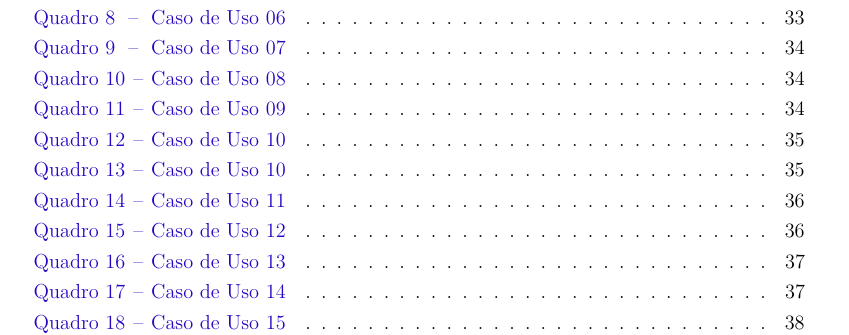
\includegraphics[width=0.9\textwidth]{erros/erros_lista_quadros.png}}
    \fonte{Trecho de um trabalho com o erro (omitida autoria propositadamente).}
\end{figure}

\begin{figure}[htb]
    \centering
	\caption{\label{fig_erros_lista_quadros_2}Exemplo de Lista de quadros com erro nos títulos}
	\frame{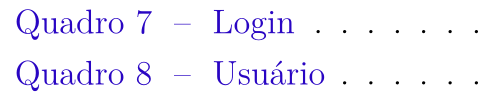
\includegraphics{erros/quadros_login_usuario.png}}
    \fonte{Trecho de um trabalho com o erro (omitida autoria propositadamente).}
\end{figure}



\subsection{Erros em tabelas e quadros}
\label{sub-erros-tabelas}
A \autoref{tabelas-e-quadros} demonstra como devemos formatar corretamente tabelas e quadros (e também indica quando devemos utilizar cada tipo de ilustração), a \autoref{tabela-errada} mostra diversos erros comuns que encontramos em tabelas e quadros, e as Tabelas \ref{tabela-correta-equipamento} e \ref{tabela-correta-servicos} mostram os mesmos dados apresentados de uma forma correta. Uma tabela formatada corretamente permite a leitura e comparação dos dados de forma mais fácil. Observe a lista de erros da \autoref{tabela-errada} :


\begin{itemize}
    \item \errado{formatação de bordas como um quadro e não como tabela};

    \item \errado{títulos sem negrito dificultando a sua leitura e identificação};
    
    \item \errado{não limitar tamanho de coluna que tem dados grandes de forma a estourar o espaço disponível};
    
    \item \errado{números não estão alinhados a direita};
    
    \item \errado{itens sem ordem especifica}, \certo{os itens devem vir em uma ordem lógica ou ordem alfabética};
    
    \item \errado{inconsistência de precisão, em uma célula o valor tem duas casas decimais e em outras não possuem casas decimais};
    
    \item \errado{mistura de dados de situações diferentes (ex: custo único e custo mensal sem normalização)};
    
    \item \errado{repetição do R\$ mesmo tendo ele no título da coluna}.
\end{itemize}

% Essa tabela além dos erros na colocação dos dados também está "estourando" a margem pois não está quebrando o texto um caso muito comum nos documentos que recebemos... 
\begin{table}[thb]
\centering
\ABNTEXfontereduzida
\caption{Valores de equipamentos (formação de forma errada e passando da margem)}
\label{tabela-errada}
\begin{tabular}{|l|c|l|l|}
\hline
Equipamento/Serviço & Valor Unitário R\$ & Quantidade & Valor Total R\$ \\ \hline
Teclado     & R\$60          & 2          & R\$120     \\ \hline
Monitor     & R\$:600          & 2          & R\$ 1200,00     \\ \hline
Internet     & R\$220          & 1          & R\$ 220     \\ \hline
Texto muito muito grande que deveria ser quebrado   & R\$120          & 1          & R\$ 120     \\ \hline
\end{tabular}
	\fonte{Os Autores.}
\end{table}

\begin{table}[]
\centering
\ABNTEXfontereduzida
\caption{Valores de equipamentos - Compra (formatada corretamente)}
\label{tabela-correta-equipamento}
\begin{tabular}{p{5.0cm}rrr}
\hline
\thead{Equipamento} & \thead{Valor\\Unitário\\R\$} & \thead{Quantidade} & \thead{Valor\\Total\\ R\$} \\ \hline
Monitor     & 600,00          & 2          & 1200,00     \\ 
Teclado     & 60,00          & 2          & 120,00     \\ 
Texto muito muito grande que deveria ser quebrado     & 220,00          & 1          & 220,00     \\ 
\hline
\textbf{TOTAL} & & & 1540,00 \\
\hline
\end{tabular}
\fonte{Os autores.}
\end{table}

\begin{table}[]
\centering
\ABNTEXfontereduzida
\caption{Valores de equipamentos - Mensal (formatada corretamente)}
\label{tabela-correta-servicos}
\begin{tabular}{lrrr}
\hline
\thead{Serviço} & \thead{Valor Unitário R\$} & \thead{Quantidade} & \thead{Valor Mensal R\$} \\ \hline
Internet     & 120,00          & 1          & 120,00     \\ \hline
\end{tabular}
\fonte{Os autores.}
\end{table}

Também é necessário cuidado em termos de formatação das ilustrações em termos de consistência e quebras :

\begin{itemize}
    
    \item \errado{quadros que devem representar o mesmo tipo de informação com formatação diferente}, uma maneira simples de garantir a padronização da formatação é utilizar o recurso de criação de comandos no {\LaTeX}, dessa forma todos elementos serão apresentados de forma consistente;

    \item \errado{utilização de \index{longtable}longtable sem necessidade} quebrando um quadro ou tabela que poderia ser apresentado em uma única página, quando o quadro ou tabela for maior que uma página a melhor maneira é quebrar em quadros que agrupem as informações de forma consistente.

\end{itemize}

\todo[inline]{gerar figura demonstrando erro do longtable com tabelas pequenas que ficam quebradas em diferentes páginas}    


Em quadros pequenos detalhes podem fazer uma grande diferença na apresentação de informação, como pode ser observado nos Quadros \ref{quadro-poluido},  \ref{quadro-poluido-limpo-desalinhado} e \ref{quadro-poluido-limpo} :

\begin{itemize}
    \item \errado{O \autoref{quadro-poluido} foi montado com textos que não facilitam a leitura};
    
    \item \errado{O \autoref{quadro-poluido-limpo-desalinhado} teve uma melhora mas sem centralização das informações};

    \item \certo{O \autoref{quadro-poluido-limpo} apresenta a mesma informação do de forma mais limpa e facilitando a leitura}.
\end{itemize}



\begin{quadro}[thb]
\centering
\ABNTEXfontereduzida
\caption{Distribuição de Atividades (poluído, difícil de ler) }
\label{quadro-poluido}
\begin{tabular}{|l|c|c|c|c|}
\hline
\thead{Responsável} & \thead{Atividade 1} & \thead{Atividade 2} & \thead{Atividade 3} & \thead{Atividade 4} \\
\hline
%
Pessoa 1 & SIM         & NÃO         & NÃO         & SIM         \\
\hline
Pessoa 2 & SIM         & NÃO         & SIM         & NÃO         \\
\hline
Pessoa 3 & NÃO         & SIM         & NÃO         & NÃO         \\
\hline
Pessoa 4 & NÃO         & SIM         & SIM         & NÃO        \\
\hline
\end{tabular}
\fonte{Os autores.}
\end{quadro}


\begin{quadro}[thb]
\centering
\ABNTEXfontereduzida
\caption{Distribuição de Atividades (sem centralização)}
\label{quadro-poluido-limpo-desalinhado}
\begin{tabular}{|l|l|l|l|l|}
\hline
\thead{Responsável} & \thead{Atividade 1} & \thead{Atividade 2} & \thead{Atividade 3} & \thead{Atividade 4} \\
\hline
Pessoa 1 & \circlemark       &          &             & \circlemark         \\
\hline
Pessoa 2 & \circlemark       &          & \circlemark      &          \\
\hline
Pessoa 3 &          & \circlemark         &             &          \\
\hline
Pessoa 4 &          & \circlemark         & \circlemark      &         \\
\hline
\end{tabular}
\fonte{Os autores.}
\end{quadro}


\begin{quadro}[thb]
\centering
\ABNTEXfontereduzida
\caption{Distribuição de atividades (de maneira mais clara e simples)}
\label{quadro-poluido-limpo}
\begin{tabular}{|l|c|c|c|c|}
\hline
\thead{Responsável} & \thead{Atividade 1} & \thead{Atividade 2} & \thead{Atividade 3} & \thead{Atividade 4} \\
\hline
Pessoa 1 & \circlemark       &          &             & \circlemark         \\
\hline
Pessoa 2 & \circlemark       &          & \circlemark      &          \\
\hline
Pessoa 3 &          & \circlemark         &             &          \\
\hline
Pessoa 4 &          & \circlemark         & \circlemark      &         \\
\hline
\end{tabular}
\fonte{Os autores.}
\end{quadro}


Utilizar corretamente a área do documento também pode fazer uma grande diferença em termos de espaço. O \autoref{quadro-descritivo-ruim} mostra que se não utilizarmos a área completa de impressão o quadro fica muito grande e difícil de ser posicionado. Os mesmos dados são apresentados no \autoref{quadro-descritivo-melhorado}, utilizando somente o tamanho necessário para os dados e títulos.


\todo[inline]{Completar o texto com mais informações sobre formatação dos quadros}
\begin{quadro}[thb]
\centering
\ABNTEXfontereduzida
\caption{Detalhamento dos itens (ruim)}
\label{quadro-descritivo-ruim}
\begin{tabular}{ | l | p{5.5cm} | l | }
\hline
\thead{Identificador pequeno} & \thead{Descrição} & \thead{Referencia} \\
\hline
XX01 & \lipsum[1]  & ZZ01  \\
\hline
XX02  & bla bla bla & KK02  \\
\hline
XX03 &  bla bla bla & MM03  \\
\hline
\end{tabular}
\fonte{Os autores.}
\end{quadro}


\begin{quadro}[thb]
\centering
\ABNTEXfontereduzida
\caption{Detalhamento dos itens (melhorado)}
\label{quadro-descritivo-melhorado}
\begin{tabular}{ | l | p{12.0cm} | l | }
\hline
\thead{Ident. \\
pequeno} & \thead{Descrição} & \thead{Ref.} \\
\hline
XX01 & \lipsum[1]  & ZZ01  \\
\hline
XX02  & bla bla bla & KK02  \\
\hline
XX03 &  bla bla bla & MM03  \\
\hline
\end{tabular}
\fonte{Os autores.}
\end{quadro}




\subsection{Erros na utilização de referencias}
\label{erros-referencias}

Um trabalho acadêmico deve ser baseado em informações confiáveis, artigos acadêmicos e livros são uma boa fonte de informações confiáveis pois passam por um processo de validação por especialistas antes de sua publicação. Os alunos do \ac{ifsp} tem acesso a diversos livros pela biblioteca online da Editora  Pearson (acessível a partir do \ac{suap}) e também ao serviço de periódicos da \ac{capes} \footnote{\url{http://periodicos.capes.gov.br/}} utilizando a opção \enquote{Acesso CAFE}.

Sempre que possível deve ser utilizada uma referencias primária, ou seja a referencia original da informação, somente quando existir a impossibilidade de acesso a obra original ou a obra original é disponibilizada em uma língua que não seja possível de ler que devemos utilizar as referencias secundárias.

Em alguns casos uma referencia utilizando endereço web pode ser necessária, nesse caso é recomendável manter essas referencias via  Web Archive, de forma a garantir que o leitor tenha acesso ao estado original da referencia utilizada, já que a maioria dos sites normalmente não armazenam histórico de alterações e também alguns sites desaparecem entre a entrega do seu trabalho e a leitura por outras pessoas.

Utilizando o {\LaTeX} parte do processo de tratamento das referencias é simplificado utilizando o padrão bibtex que é disponibilizado em diversas ferramentas, mas a \ac{abnt} possui definições que não são obrigatórias em outros países o que faz com que as referencias precisem de alguns ajustes.


\begin{itemize}
    \erradocerto{utilizar o formato de citação errada em fontes, ver \autoref{referencias}}{Fonte: \cite{alcarde1996}.}{Fonte: \citeonline{alcarde1996}.}

    \erradocerto{Erro na definição de publicações de organizações/empresas (ver definições de NBR6028 no arquivo .bib)}{sem utilizar \textbf{\textit{organization}} \cite{NBR6028:2003-errado}}{utilizando \textbf{\textit{organization}} \cite{NBR6028:2003}}

    \erradocerto{Erro na definição de nomes com acentuação}{...texto \cite{acentuacao-ok}.}{...texto \cite{acentuacao-errada}.}
    
\IfPackageLoaded{biblatex}{%
\explicacaoErro{O erro referente a erro de acentuação só pode ser demonstrado quando o documento foi compilado com \mostraPacoteLaTeX{abntex2cite} e este documento foi compilado com \mostraPacoteLaTeX{biblatex}}
}{}
\end{itemize}



\subsection{Erros em citações indiretas}
\label{erros-citacoes-indiretas}

As citações devem ficar em formato compatível com o texto onde ela estão localizadas. O tipo de citação deve ser escolhido corretamente para isso. O tipo de citação mais utilizado é a citação indireta, onde o o texto é escrito com suas próprias palavras e a referencia indicada.

Utilizar o texto de outra pessoa sem a citação da forma correta é  considerado plágio.

\todo[inline]{informações sobre plágio :  \url{https://dicas.ivanfm.com/aulas/textos/plagio.html}}



O formato deve ser escolhido de acordo com o contexto utilizado :

\begin{itemize}
    \erradoerradocerto{utilizar o formato de citação errada, ver \autoref{referencias}}{de acordo com \cite{alcarde1996} ...}{de acordo com \citeauthor{alcarde1996} ...}{de acordo com \citeonline{alcarde1996}...}

% NBR 10520:2002 ver exemplos em 6.1.5
    \erradoerradocerto{erro ao citar em final do paragrafo, o ponto final fica após a citação }{...texto.\cite{alcione1988} Texto}{\cite{alcione1988} Texto.....}{...texto \cite{alcione1988}. Texto....}


\end{itemize}


\subsection{Erros em citações diretas}
\label{erros-citacoes-diretas}

A \ac{abnt} define formatos específicos para citações diretas (aquelas onde é necessário colocar exatamente o que foi escrito pelo autor referenciado), citações curtas e citações longas (mais de 3 linhas). A citação curta é feita diretamente durante a escrita do texto, mas a citação longa deve ser feita de uma forma especifica. A \autoref{fig_citacao_longa_errada} demonstra a forma errada da citação e a \autoref{fig_citacao_longa_certa} mostra o formato correto para a citação longa.

É importante dar preferencias para citação indireta onde você escreve com suas próprias palavras e indica a fonte da informação. Somente em casos onde o texto original precisa ser utilizado que a citação direta deve ser utilizada.

\begin{figure}[hbt]
    \centering
    \caption{Citação direta longa - incorreta}
    \label{fig_citacao_longa_errada}
\fbox{\begin{minipage}{\textwidth}
Podemos observar que historicamente existem problemas que devem ser tratados: 
    ``\textoFalso{Simulação de Citação}{5}'' \cite{ETAL5}.
\end{minipage}}
\fonte{Os Autores.}
\end{figure}

\begin{figure}[htb]
    \centering
    \caption{Citação direta longa - correta}
    \label{fig_citacao_longa_certa}
    \fbox{\begin{minipage}{\textwidth}
Podemos observar que historicamente existem problemas que devem ser tratados: 
    \begin{citacao}
    \textoFalso{Simulação de Citação}{5} \cite{ETAL5}
    \end{citacao}
\end{minipage}}
\fonte{Os Autores.}
\end{figure}


\subsection{Erros em Apêndices e Anexos}
\label{erros-apendices-e-anexos}

Apesar de parecidos Apêndices e Anexos tem características diferentes. Como Apêndices são colocados documentos adicionais do autor e como Anexos documentos gerados por outras pessoas ou instituições. Mas é necessário cuidado ao escolher o que será colocado nessas áreas do trabalho. Elementos como leis e outros documentos que podem ser facilmente encontrados não devem ser incluídos, mas referenciados (principalmente utilizando a ferramenta \url{https://web.archive.org} que permite salvar a situação de um endereço web em um momento especifico).  

